\documentclass[fr, license=none]{../../../../../../eplexam}

\usepackage{../../../../../../eplcode}

\lstset{language={C}}

\hypertitle{Systèmes informatiques}{4}{SINF}{1252}{2016}{Septembre}{Majeure}
{John de Wasseige\and Gilles Peiffer}
{Olivier Bonaventure}

% TODO : Partie théorique, vient avant INGInious (where are the questions though...).

Le syllabus est accessible depuis l'URL \url{http://sites.uclouvain.be/SystInfo}.

\textbf{Les pages de manuel sont accessibles depuis les URLs suivants :}
\begin{itemize}
     \item \url{http://sites.uclouvain.be/SystInfo/manpages/man1} (commandes);
     \item \url{http://sites.uclouvain.be/SystInfo/manpages/man2} (appels systèmes);
     \item \url{http://sites.uclouvain.be/SystInfo/manpages/man3} (fonctions librairies).
\end{itemize}

\textbf{Attention:} veuillez utiliser la version \textbf{\html{}} du syllabus.

\section{Traduction de code assembleur}

La fonction suivante a été écrite en assembleur.
Traduisez-la en une version équivalente en \clang{}.
Votre fonction doit nécessairement avoir comme nom \texttt{mp}.

\begin{lstlisting}[language={[x86masm]Assembler}, emph={\$,\%,(,),movl,cmpl,addl,subl},emphstyle={\color{blue}\bfseries}]
mp:
  subl $8, %esp
  movl 16(%esp), %edx
  movl 12(%esp), %ecx
  movl %ecx,%eax
  addl %ecx,%ecx
  addl %eax,%ecx
  cmpl %edx,%ecx
  jle m1
  movl %edx, %eax
  addl $8, %esp
  ret
 m1:
  movl %ecx, %eax
  addl $8, %esp
  ret

\end{lstlisting}

\begin{solution}

\begin{lstlisting}
int mp(int c, int d)
{
    int a = c;
    c += c;
    c += a;
    if (d < c)
    {
        return d;
    }
    else
    {
        return c;
    }
}

\end{lstlisting}

\end{solution}

\section{Liste doublement chaînée}

Une liste doublement chaînée est implémentée comme suit.
Notez que suite à l'implémentation de la fonction
\texttt{list\_init}, le premier noeud de la liste est toujours vide
et ne contient aucune donnée.
Vous devez implémenter la fonction \texttt{delete} dont les spécifications vous sont fournies.

\begin{lstlisting}
#include<stdio.h>
#include<stdlib.h>

// Noeud de la liste chaînée
typedef struct Node {
        int data;
        struct Node *next;
        struct Node *prev;
} node;

// La liste doublement chaînée. Cette liste comprend un premier
// noeud vide qui ne contient pas de donnée utile. Les données
// utiles sont stockées à partir du second noeud.

typedef struct List {
  node *start;  // pointe toujours vers le premier élément
  node *tail;   // pointe toujours vers le dernier élément
} list;

/*
 * @pre l!=NULL
 * @post a initialisé la liste doublement chaînée l. Une liste vide
 *       contient toujours un premier noeud qui est vide
 *       et dont les pointeurs next et prev pointent vers NULL
 *       retourne 0 en cas de succès, -1 en cas d'erreur
 */

int list_init(list *l) {

  l->start=malloc(sizeof(node));
  if(l->start==NULL)
    return -1;
  l->start->next=NULL;
  l->start->prev=NULL;
  l->start->data=-1;
  l->tail=l->start;
  return 0;
}

/*
 * @pre l!=NULL
 * @post insert à la fin de la liste un noeud content la donnée data
 *       retourne -1 en cas d'erreur, 0 sinon
 */
int insert(list *l, int data)
{
  node *pointer;
  pointer = (node *)malloc(sizeof(node));
  if(pointer==NULL)
    return -1;
  l->tail->next=pointer;
  pointer->prev=l->tail;
  l->tail=pointer;
  pointer->data = data;
  pointer->next = NULL;
  return 0;
}

/*
 * @pre l!=NULL
 * @post a retiré de la liste l tous les noeuds dont la donnée
 *       est key
 *       retourne le nombre de noeuds retirés, -1 en cas d'erreur
 */
int delete(list *l, int key)
{

\end{lstlisting}

\begin{solution}

\begin{lstlisting}
node* runner = l->start->next;
int counter = 0;

if (runner == NULL) {
    return counter;
}

while (runner->next != NULL) {
    if (runner->data == key) {
        runner->next->prev = runner->prev;
        runner->prev->next = runner->next;
        
        node *del = runner;
        runner = runner->next; 
        
        del->prev = NULL;
        del->next = NULL;
        free(del);
        counter++;
    } else {
		runner = runner->next;
    }
}
 if (runner->data == key) {
     runner->prev->next = NULL;
     l->tail = runner->prev;
     free(runner);
     counter++;
 }
return counter;
\end{lstlisting}

\end{solution}

\section{Producteurs/Consommateurs}

\begin{figure}[!htb]
  \centering
  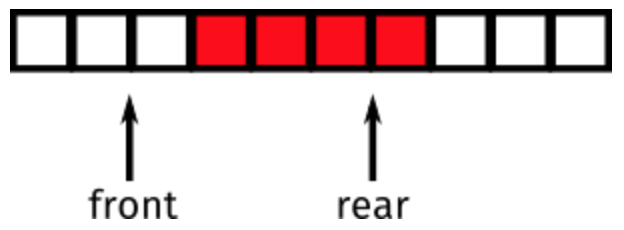
\includegraphics[width=0.5\textwidth]{prodcons.png}
\end{figure}

\subsection{Fonction \texttt{insert}}

Une librairie supportant un buffer partagé utilisé pour résoudre le problème des
``Producteurs/Consommateurs'' est implémentée comme suit.

\begin{lstlisting}
typedef struct {
    int *buf;          /* Buffer partagé */
    int n;             /* Nombre de slots dans le buffer */
    int front;         /* buf[(front+1)%n] est le premier élément */
    int rear;          /* buf[rear%n] est le dernier */
    sem_t mutex;       /* Protège l'accès au buffer */
    sem_t slots;       /* Nombre de places libres */
    sem_t items;       /* Nombre d'items dans le buffer */
} sbuf_t;

/*
 * @pre sp!=NULL, n>0
 * @post a construit un buffer partagé contenant n slots
 */
void sbuf_init(sbuf_t *sp, int n)
{
    sp->buf = calloc(n, sizeof(int));
    sp->n = n;                       /* Buffer content les entiers */
    sp->front = sp->rear = 0;        /* Buffer vide si front == rear */
    sem_init(&sp->mutex, 0, 1);      /* Exclusion mutuelle */
    sem_init(&sp->slots, 0, n);      /* Au début, n slots vides */
    sem_init(&sp->items, 0, 0);      /* Au début, rien à consommer */
}

/*
 * @pre sp!=NULL
 * @post libère le buffer
 */
void sbuf_clean(sbuf_t *sp)
{
    free(sp->buf);
}

/* @pre sp!=NULL
 * @post ajoute item à la fin du buffer partagé. Ce buffer est géré
 *       comme une queue FIFO
 */
void sbuf_insert(sbuf_t *sp, int item)
{
  // à compléter

\end{lstlisting}

\begin{solution}

\begin{lstlisting}
sem_wait(&(sp->slots));
sem_wait(&(sp->mutex));

sp->rear = (sp->rear+1)%sp->n;
sp->buf[sp->rear] = item;

sem_post(&(sp->mutex));
sem_post(&(sp->items));

\end{lstlisting}

\end{solution}

\subsection{Fonction \texttt{remove}}

Implémentez ici la fonction suivante

\begin{lstlisting}
/* @pre sbuf!=NULL
 * @post retire le dernier item du buffer partagé
 */
int sbuf_remove(sbuf_t *sp)
{

\end{lstlisting}

\begin{solution}

\begin{lstlisting}
sem_wait(&(sp->items));

int val;

sem_wait(&(sp->mutex));
sp->front = (sp->front + 1)%sp->n;

val = sp->buf[sp->front];
sem_post(&(sp->mutex));

sem_post(&(sp->slots));
return val;

\end{lstlisting}

\end{solution}

\section{Stockage d'un vecteur de réels dans un fichier}

Afin de compléter une librairie permettant de stocker et de manipuler
des vecteurs contenant des réels en les plaçant dans des fichiers plutôt qu'en mémoire,
vous devez implémenter la fonction \texttt{swap} en utilisant uniquement les appels systèmes suivants:
\lstinline|open|, \lstinline|read|, \lstinline|write| et \lstinline|close|.
Le code de la fonction \texttt{create} de la librairie vous est fournie.

\begin{lstlisting}
#include <fcntl.h>
#include <sys/types.h>
#include <sys/stat.h>
#include <sys/uio.h>
#include <unistd.h>
#include <stdlib.h>
#include <stdio.h>

/*
 * Implementation de vecteurs en utilisation des fichiers
 * La donnée à l'indice zéro correspond aux sizeof(double)
 * premiers bytes du fichier, la deuxième aux suivantes, etc.
 * La taille d'un tel fichier est toujours un multiple
 * entier de sizeof(double)
 */

/*
 * @pre *filename!=NULL, size>0
 * @post construit un fichier contenant size double à la valeur val
 *       retourne le nombre de données écrites, -1 en cas d'erreur
 */
int create(char *filename, int size, double val) {

  int err;
  int fd=open(filename,O_RDWR|O_CREAT,S_IRUSR|S_IWUSR);
  if(fd==-1) {
    return -1;
  }
  for(int i=0; i<size; i++) {
    err=write(fd,(void *) &val, sizeof(double));
    if(err<0) {
       err=close(fd);
       return(-1);
     }
   }
   err=close(fd);
   if(err==-1)
     return err;
   else
     return size;
 }

/*
 * @pre filename!=NULL, 0 <= i*sizeof(double) < taille fichier,
 *       0 <= j*sizeof(double) < taille fichier
 * @post échange les données aux indices i et j dans
 *       le vectorfile (0 est le premier indice)
 *       retourne 0 en cas de succès, -1 si erreur
 */

int swap(char *filename, int i, int j) {

\end{lstlisting}

\begin{solution}

\begin{lstlisting}
if(i==j)
{
    return 0;
}

int err;
int fd;

int max_idx = i;
int min_idx = j;
if (i < j) {
    max_idx = j;
    min_idx = i;
}

fd = open(filename, O_RDONLY, S_IRUSR|S_IWUSR);
if (fd == -1) {
    return -1;
}

double val[max_idx+1];
for(int k=0; k <= max_idx; k++) {
    err = read(fd, (void *) &(val[k]), sizeof(double));
    if (err < 0) {
        err = close(fd);
        return(-1);
    }
}
if(close(fd) == -1) {
    return err;
}

fd = open(filename, O_WRONLY, S_IRUSR|S_IWUSR);
if (fd == -1) {
    return -1;
}

double new_val;
for(int k=0; k <= max_idx; k++) {
    if (k == min_idx) {
        new_val = val[max_idx];
    } else if (k == max_idx) {
        new_val = val[min_idx];
    } else {
        new_val = val[k];
    }
    err = write(fd, (void *) &new_val, sizeof(double));
    if (err < 0) {
        err = close(fd);
        return(-1);
    }
}
if(close(fd) == -1) {
    return err;
}

return 0;
\end{lstlisting}

\end{solution}

\end{document}
